\chapter*{Chapter Dependencies}

\begin{center}
  \tikzstyle{boxed}=[rectangle, draw=black, minimum width=1cm,rounded corners=0.2cm, thick]
  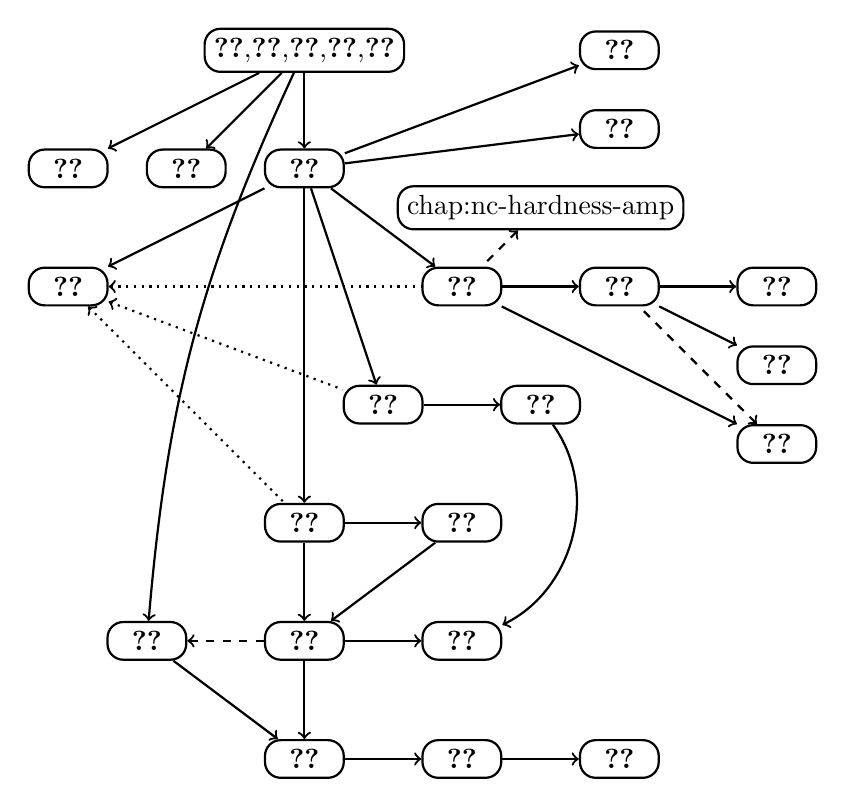
\begin{tikzpicture}[transform shape, scale=1]
    \node[boxed] (c2-5) at (0,-1.5) {\ref{chap:intro},\ref{chap:notation},\ref{chap-vpvnp},\ref{chap:binom-estimates},\ref{chap:structural-results}};

    \node[boxed] (classical) at (-3,-3) {\ref{chap:gen-ckt-formulas}}
    edge[<-,thick] (c2-5);

    \node[boxed] (dc) at (-1.5,-3) {\ref{chap:dc}}
    edge[<-,thick] (c2-5);

    \node[boxed] (simpleLBs) at (0,-3) {\ref{chap:simpleLBs}}
    edge[<-,thick] (c2-5);
    
    \node[boxed] (SW) at (1,-6) {\ref{chap:d3SW}}
    edge[<-, thick] (simpleLBs);

    \node[boxed] (GK) at (3, -6) {\ref{chap:GK}}
    edge[<-, thick] (SW);

    \node[boxed] (PDM) at (2, -4.5) {\ref{chap:evalDim}}
    edge[<-, thick] (simpleLBs);

    \node[boxed] (multmodels) at (4, -4.5) {\ref{chap:multilinear}}
    edge[<-, thick] (PDM);

    \node[boxed] (CILM) at (3,-3.5) {\autoref{chap:nc-hardness-amp}}
    edge[<-, thick, dashed] (PDM);
    
    \node[boxed] (multi-k) at (6, -4.5) {\ref{chap:multi-k-ic}}
    edge[<-, thick] (multmodels);

    \node[boxed] (DMPY) at (6, -5.5) {\ref{chap:DMPY}}
    edge[<-, thick] (multmodels);

    \node[boxed] (tensorrank) at (6,-6.5) {\ref{chap:tensorrk}}
    edge[<-, dashed, thick] (multmodels)
    edge[<-, thick] (PDM);

    \node[boxed] (monABPCktSep) at (4, -1.5) {\ref{chap:monABPCktSep}}
    edge[<-, thick] (simpleLBs);

    \node[boxed] (monABPCktSep) at (4, -2.5) {\ref{chap:monVPVNP}}
    edge[<-, thick] (simpleLBs);

    \node[boxed] (SPDs) at (0, -7.5) {\ref{chap:d4-bottomfanin}}
    edge[<-, thick] (simpleLBs);
    edge[<-, thick,dashed] (SW);

    \node[boxed] (PSPDs) at (2, -7.5) {\ref{chap:d4hom}}
    edge[<-, thick] (SPDs);

    \node[boxed] (PSPDsummary) at (0,-9) {\ref{chap:SPD_summary}}
    edge[<-, thick] (PSPDs)
    edge[<-, thick] (SPDs);

    \node[boxed] (PSPDEval) at (2,-9) {\ref{chap:PSPD-more}}
    edge[<-, thick] (PSPDsummary)
    edge[<-, thick, bend right=50] (GK);

    \node[boxed] (d3chasm) at (-2,-9) {\ref{chap:d3nonhom}}
    edge[<-, thick, bend left=10] (c2-5)
    edge[<-, dashed, thick] (PSPDsummary);

    \node[boxed] (d3lowarity) at (0,-10.5) {\ref{chap:lowbottomfanind3}}
    edge[<-, thick] (PSPDsummary)
    edge[<-, thick] (d3chasm);
    
    \node[boxed] (d4lowarity) at (2,-10.5) {\ref{chap:d4lowarity}}
    edge[<-, thick] (d3lowarity);

    \node[boxed] (llalgrank) at (4,-10.5) {\ref{chap:lowAlgRank}}
    edge[<-, thick] (d4lowarity);

    \node[boxed] (subrankbarrier) at (-3,-4.5) {\ref{chap:subadditive-rank-barrier}}
    edge[<-, thick] (simpleLBs)
    edge[<-, thick, dotted] (SW)
    edge[<-, thick, dotted] (PDM)
    edge[<-, thick, dotted] (SPDs);
\end{tikzpicture}
\end{center}

\noindent
{\tikz[baseline=-0.5ex]{\draw[->,thick] (0,0) -- (1,0);}}\;: Dependency

\noindent
{\tikz[baseline=-0.5ex]{\draw[->,dashed,thick] (0,0) -- (1,0);}}\;: Not a dependency, but recommended

\noindent
{\tikz[baseline=-0.5ex]{\draw[->,dotted, thick] (0,0) -- (1,0);}}\;: Familiarity would be helpful

%%% Local Variables:
%%% mode: latex
%%% TeX-master: "fancymain"
%%% End:
